\documentclass[12pt,a4paper]{report}
\usepackage{graphicx}
\usepackage[spanish]{babel}
\begin{document}
\begin{titlepage}

	\centering
	
\includegraphics[width=0.5\textwidth]{../images/ciateq.jpg}\par\vspace{1cm}
	\vspace{1cm}
	{\scshape\Large Sistemas Operativos (Linux)\par}
	\vspace{1.5cm}
	{\huge\bfseries Notas de clases\par}
	\vspace{2cm}
	{\Large\itshape H\'{e}ctor Edmundo Ram\'{i}rez G\'{o}mez\par}
	\vfill
	Profesor\par
	\textsc{Mtro. Jayro Santiago Paz}
	\vfill

	{\large \date sOctubre 2017\par}
\end{titlepage}

\chapter{Sistema Operativo}

\section{?`Qu\'{e} es un sistema operativo?}
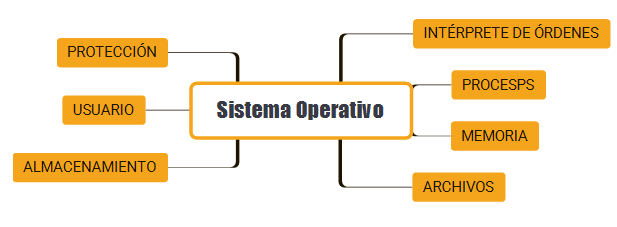
\includegraphics[width=1\textwidth]{../images/sistema_operativo.png}
Es el software principal de un sistema que gestiona los recursos del hardware y provee servicios a las aplicaciones.
%\centering
\par\vspace{1cm}
\begin{itemize}
	\item Procesos
	\begin{itemize}
	\item Crear y destruir procesos
	\item Parar y reanudar
	\item Comunicaci\'{o}n y sincronizaci\'{o}n
	\end{itemize}
	\item Memoria
	\begin{itemize}
	\item Conocer qu\'{e} partes de la memoria est\'{a}n siendo utilizadas
	\item Decidir
	\item Asignar o liberar	
	\end{itemize}
	\item Almacenamiento
	\begin{itemize}
	\item Planificar los discos
	\item Gestionar el espacio
	\item Asignar el almacenamiento	
	\end{itemize}
	\item Usuario
	\begin{itemize}
	\item Gestionar el almacenamiento temporal de E/S y servir las interrupciones de los dispositivos de E/S	
	\end{itemize}
	\item Archivos
	\begin{itemize}
	\item Construir, eliminar
	\item Ofrecer funciones para la manipulaci\'{o}n
	\item Establecer correspondencia
	\item Realizar copias de seguridad	
	\end{itemize}
	\item Protecci\'{o}n
	\begin{itemize}
	\item Autorizaci\'{o}n y autenticaci\'{o}n
	\item Especificar los controles de seguridad
	\item Forzar el uso de mecanismos de protecci\'{o}n	
	\end{itemize}
\end{itemize}

\chapter{GNU/Linux}
\section{Caracter\'{i}sticas de GNU/Linux}
El n\'{u}cleo o kernel del sistema operativo
\begin{itemize}
\item Multiusuario
\item Multiplataforma
\item Multiprocesador
\item Arquitectura SMP (Symmetric Multiprocessing)
\end{itemize}
Mulltitarea
\begin{itemize}
\item Cooperativa en Windows
\item Apropiativa en Linux
\item Real: M\'{u}ltiples procesos ejecut\'{a}ndose en m\'{u}ltiples procesadores
\end{itemize}
Estructura b\'{a}sica de Linux
\begin{itemize}
\item N\'{u}cleo
\item Shell\\
Interfaz entre el n\'{u}cleo y el usuario
\begin{itemize}
\item Shell Boorne (sh)
\item S-shell (csh)
\item Shell job (jsh)
\item Shell korn (ksh)
\item Boorne Again Shell (bash)
\end{itemize}
\item Sistema de archivos\\
Para Linux todo es archivos, hay diferentes tipos de archivos los cuales son:
\begin{itemize}
\item ext2
\item ext3
\item ext4
\item ReiserFS
\item swap (como memoria de intercambio)
\end{itemize}
Para ver el file-system se utiliza el siguiente comando:\\
\$tree -L 1
\item Utilidades
\end{itemize}
\section{Interfaces de Linux}
\begin{itemize}
\item Gnome
\item KDE Plasma
\item Mint Cinnamon
\item Lxqt
\item Mate
\item Unity Ubuntu
\item Xface
\end{itemize}
\section{Distribuciones}
\begin{itemize}
\item Mandriva
\item Suse
\item Ubuntu
\item Kubuntu
\item CentOS
\item Debian
\item Fedora
\item xUbuntu
\item ArchLinux
\item semiCodoe
\item Elementary
\item MoonOS
\item Quimo
\end{itemize}

\chapter{Redirecciones y Tuber\'{i}as}
\section{Tipos de tuber\'{i}as}
\begin{itemize}
\item Entrada est\'{a}ndar (tipo 0)
\item Salida est\'{a}ndar (tipo 1)
\item Error est\'{a}ndar (tipo 2)
\end{itemize}

\chapter{Fork}
\begin{itemize}
\item Es una copia exacta
\item Mismas variables
\item Mismos ficheros abiertos
\item Variables independientes
\item fork() retorna 0 al nuevo proceso
\item fork() retorna un valor positivo (PID) al proceso padre
\end{itemize}

\chapter{Android}
Es un entorno dde SW construido para dispositivos móviles
\begin{itemize}
\item SO basado en el kernel de Linux
\item App se desarrolla en java
\end{itemize}
\section{Aplicaciones}
\begin{itemize}
\item Primer plano (foreground): muestran una UI
\item Segundo plano (background): Servicios
\item Widget (Appwidget): Aplicaciones de pequeña UI
\end{itemize}

\section{Framework}
Conjunto de herramientas de desarrollo
\begin{itemize}
\item Activity manager
\item Window manager
\item Telephone
\item Content provider
\item View System
\item Location Manager
\item Notification
\end{itemize}

\section{Librerías Nativas}
\begin{itemize}
\item Escritas en C/C++
\item Código abierto
\item System C
\item Media Framework (Open Core)
\item Surface Manager
\item Webkit
\item Open GL
\item SQLite
\end{itemize}

\section{Android runtime}
\begin{itemize}
\item Librerías core
\item Dalvik
\end{itemize}

\section{Nucleo de Linux}
\begin{itemize}
\item Controladores del HW
\item Procesos
\item Memoria
\item seguridad
\item Red
\item Gestión de energía
\end{itemize}
\end{document}
